\documentclass[a4paper,12pt]{report}

% Page layout
\usepackage[left=2.5cm,right=2.5cm,top=2.5cm,bottom=2.5cm]{geometry}

% Font and text
\usepackage[afrikaans,english]{babel}
\usepackage{microtype}
\usepackage{setspace}
\usepackage{lmodern}
\usepackage{siunitx}
\usepackage{tcolorbox}
% \usepackage[scaled=.96]{XCharter}
\usepackage[scaled=.96]{caladea}  % font required by Stellenbosch University
\usepackage[scaled=.96,lf]{carlito}  % the scaling makes the math the same height
\renewcommand*\oldstylenums[1]{\carlitoOsF #1}
\newcommand{\myemph}[1]{{\sffamily\bfseries#1}}
\sloppy
\onehalfspacing

% Headings
\usepackage[raggedright,sf,bf]{titlesec}
\usepackage[margin=\the\parindent,small,bf,sf]{caption}
\titlelabel{\thetitle.\ }
\titleformat{\chapter}[display]{\huge\bfseries\sffamily}{\chaptertitlename\ \thechapter}{15pt}{\Huge \raggedright}
\titlespacing*{\chapter}{0pt}{0pt}{40pt}  % remove spacing before chapter headings
\makeatletter
\let\originall@chapter\l@chapter
\def\l@chapter#1#2{\originall@chapter{{\sffamily #1}}{#2}}
\makeatother

%% Alternative headings using small-caps (comment out the top section)
%\usepackage[raggedright,bf]{titlesec}
%\usepackage[margin=\the\parindent,small,bf]{caption}
%\titlelabel{\thetitle.\ }
%\titleformat{\chapter}[display]{\huge\scshape}{\chaptertitlename\ \thechapter}{15pt}{\Huge \raggedright}
%\titlespacing*{\chapter}{0pt}{0pt}{40pt}  % remove spacing before chapter headings

% Table of contents
\let \savenumberline \numberline
\def \numberline#1{\savenumberline{#1.}}

% Figures
\usepackage{graphicx}
\usepackage{tikz}
\usepackage{pdfpages}
\usepackage{subcaption}
\setlength{\abovecaptionskip}{7.5pt}  % spacing above and below captions
\newcommand*{\WaterMark}[2][0.2\paperwidth]{\AddToShipoutPicture*{\AtTextCenter{\parbox[c]{0pt}{\makebox[0pt][c]{\includegraphics[width=#1]{#2}}}}}}

% Mathematics
\usepackage[cmex10]{amsmath}
\usepackage{amssymb}
\usepackage{cancel}
\DeclareMathOperator*{\argmax}{arg\,max}
\newcommand{\T}{^\top}
\newcommand{\tr}{\textrm{tr}}
\renewcommand{\vec}[1]{\boldsymbol{\mathbf{#1}}}
\newcommand{\defeq}{\triangleq}

% Tables
\usepackage{booktabs}
\usepackage{tabularx}
\usepackage{multirow}
\newcommand{\mytable}{
    \centering
    \small
    \renewcommand{\arraystretch}{1.2}
    }
\renewcommand{\tabularxcolumn}[1]{m{#1}}
\newcolumntype{C}{>{\centering\arraybackslash}X}
\newcolumntype{L}{>{\raggedright\arraybackslash}X}

% Header and footer
\usepackage{fancyhdr}
\pagestyle{fancy}
\fancyhf{}
\renewcommand{\sectionmark}[1]{\markright{\normalsize \thesection.\ #1}}
\fancyhead[C]{\nouppercase{\textit{\rightmark}}}
\fancyhead[RO]{\thepage}
\fancyhead[LE]{\thepage}  % double-sided printing
\fancyfoot{}
\setlength\headheight{14.5pt}
\renewcommand{\headrulewidth}{0pt}
\fancypagestyle{plain}{\fancyhead{}
                       \renewcommand{\headrulewidth}{0pt}
                       \fancyfoot[C]{\thepage}}

% Pseudo-code
\usepackage{algorithm}  % should go before \usepackage{hyperref}

% Table of contents and hyperlinks
\usepackage{hyperref}
\hypersetup{colorlinks=true,linktoc=all,citecolor=black,linkcolor=black}
\usepackage[nottoc]{tocbibind}

% Pseudo-code
\usepackage{algpseudocode}  % should go after \usepackage{hyperref}
\renewcommand{\thealgorithm}{\arabic{chapter}.\arabic{algorithm}} 
\captionsetup[algorithm]{labelfont={bf,sf},font=small,labelsep=colon}

% Bibliography
\usepackage{cite}  % automatically reorder inline citations
\bibliographystyle{IEEEtran}

% Fix titlesec issue
\usepackage{etoolbox}
\makeatletter
\patchcmd{\ttlh@hang}{\parindent\z@}{\parindent\z@\leavevmode}{}{}
\patchcmd{\ttlh@hang}{\noindent}{}{}{}
\makeatother

% Custom Packages
\usepackage{marginnote}

\newcommand{\note}[1]{%
    \marginnote{\textcolor{red}{#1}}%
}
\usepackage{parskip}

\begin{document}

% Front matter
\graphicspath{{frontmatter/fig/}}
\pagenumbering{Alph}

\begin{titlepage}
    \begin{tikzpicture}[remember picture, overlay]
        \node [opacity=1.0, anchor=center] at (current page.center) 
        {
\includegraphics[width=\paperwidth]{stb-thesis-frntp.pdf}};
    \end{tikzpicture}

	\begin{center}			
		\vfill
        \vfill
        \vfill
		{\bfseries \huge A Contrastive Approach to Weight Space Learning \par}
		\vfill
        {\large by \\[5pt]}
		{\Large {\Large D.J. Swanevelder} \par}
		\vfill
		\vfill

		{\large MSc Machine Learning/ Artificial Intelligence \par
		 Department of Applied Mathematics \par Faculty of Science \par Stellenbosch University \par}
		
		\vfill
		
		{\large {Supervisor}: Ruan van der Merwe}\par
		\vfill
		{\large November 2025}
        \vfill
	\end{center}
\end{titlepage}
 % include
\pagenumbering{roman} 
% \thispagestyle{plain}

% \vspace*{5pt}

\chapter*{Declaration}
\addcontentsline{toc}{chapter}{Declaration}

% \vspace{20pt}

% Masters (Research)
By submitting this thesis electronically, I declare that the entirety of the work contained
therein is my own, original work, that I am the sole author thereof (save to the extent explicitly
otherwise stated), that reproduction and publication thereof by Stellenbosch University will
not infringe any third party rights and that I have not previously in its entirety or in part
submitted it for obtaining any qualification.

% % PhD
% By submitting this dissertation electronically, I declare that the entirety of the work contained
% therein is my own, original work, that I am the sole author thereof (save to the extent explicitly
% otherwise stated), that reproduction and publication thereof by Stellenbosch University will not
% infringe any third party rights and that I have not previously in its entirety or in part submitted it
% for obtaining any qualification.

\vspace{35pt}

% \vspace{1cm}
\noindent
\begin{minipage}{.5\textwidth}
    \noindent
    \phantom{Date:}~\hfill\makebox[0pt][c]{December 2099}\hfill\mbox{}\\[-.5\baselineskip]
    Date:~ \dotfill\mbox{}\par
\end{minipage}

\vspace{35pt}

\vfill

% \begin{center}
    Copyright © 2099 Stellenbosch University\par
    All rights reserved
% \end{center}

\vspace{35pt}


\chapter*{Abstract}
\addcontentsline{toc}{chapter}{Abstract}
\makeatletter\@mkboth{}{Abstract}\makeatother
% TODO {abstract} 
The fundamental goal is to have system which is capable of embedding a dataset $\mathcal{D}$, the trained neural weights $W$, and the corresponding results $R$ (training and test) into a shared embedding latent space. The goal is to use the shared space, to sample from the space  conditioned on a new unseen dataset and a specified results, and decode into real weights.  The architecture is kept constant for simplicity. 
$$ p (W \mid R, \mathcal{D},\text{Arch})
$$
The way in which this will be implemented requires a few building blocks.
- Synthetic dataset generator
- Training pipeline and weight storage
- Weight Embedding
- Dataset Embedding
- Shared embedding projection

The goal of the project is to get the simplest implementation of the following up and running as fast as possible, and the evaluate the performance, then iteratively update the part of the pipeline to achieve better results. The goal is a graph, with input results (desired results) on the x-axis, measured results on the y. If the graph is somewhat linear, project is a success. 

% TODO {abstract} 

 % include
% \chapter*{Acknowledgements}
% \addcontentsline{toc}{chapter}{Acknowledgements}
\makeatletter\@mkboth{}{Acknowledgements}\makeatother
% TODO {Acknowledgements}
    I would like to thank my cat, Muffin. I also would like to thank the inventor of the incubator; without him/her, I would not be here. Finally, I would like to thank Dr Herman Kamper for this amazing report template.
% TODO {Acknowledgements}

 % include
\tableofcontents % include
%\listoffigures % include
%\listoftables % include
% \chapter*{Nomenclature\markboth{}{Nomenclature}}
\addcontentsline{toc}{chapter}{Nomenclature}
% TODO {nomeclature}
    % \vspace*{-3mm}
\subsubsection*{Variables and functions}

\begingroup
\renewcommand{\arraystretch}{1.2}
\renewcommand{\tabularxcolumn}[1]{p{#1}}
\begin{tabularx}{\textwidth}{@{}p{2.5cm}L}
    $p(x)$ & Probability density function with respect to variable $x$.\\
    $P(A)$ & Probability of event $A$ occurring.\\
    $\varepsilon$ & The Bayes error. \\
    $\varepsilon_u$ & The Bhattacharyya bound. \\
    $B$ & The Bhattacharyya distance. \\
    $s$ & An HMM state.  A subscript is used to refer to a particular state, e.g.\ $s_i$ refers to the $i^{\text{th}}$ state of an HMM. \\
    $\mathbf{S}$ & A set of HMM states. \\
    $\mathbf{F}$ & A set of frames. \\
    $\mathbf{o}_f$ & Observation (feature) vector associated with frame $f$. \\
    $\gamma_s(\mathbf{o}_f)$ & A posteriori probability of the observation vector $\mathbf{o}_f$ being generated by HMM state $s$. \\
    $\mu$ & Statistical mean vector. \\
    $\Sigma$ & Statistical covariance matrix. \\
    $L(\mathbf{S})$ & Log likelihood of the set of HMM states $\mathbf{S}$ generating the training set observation vectors assigned to the states in that set. \\
    $\mathcal{N}(\mathbf{x} | \mu, \Sigma)$ & Multivariate Gaussian PDF with mean $\mu$ and covariance matrix $\Sigma$.\\
    $a_{ij}$ & The probability of a transition from HMM state $s_i$ to state $s_j$. \\
    $N$ & Total number of frames or number of tokens, depending on the context. \\
    $D$ & Number of deletion errors. \\
    $I$ & Number of insertion errors. \\
    $S$ & Number of substitution errors. \\
\end{tabularx}
\endgroup


\newpage
\subsubsection*{Acronyms and abbreviations}

\begingroup
\renewcommand{\arraystretch}{1.2}
\begin{tabular}{@{}p{2.5cm} l}
    AE      & Afrikaans English \\
    AID     & accent identification \\
    ASR     & automatic speech recognition \\
    AST     & African Speech Technology \\
    CE      & Cape Flats English \\
    DCD     & dialect-context-dependent \\
    DNN		& deep neural network \\
    G2P     & grapheme-to-phoneme \\
    GMM     & Gaussian mixture model \\
    HMM     & hidden Markov model \\
    HTK     & Hidden Markov Model Toolkit \\
    IE      & Indian South African English \\
    IPA     & International Phonetic Alphabet \\
    LM      & language model \\
    LMS     & language model scaling factor \\
    MFCC    & Mel-frequency cepstral coefficient \\
    MLLR    & maximum likelihood linear regression \\
    OOV     & out-of-vocabulary \\
    PD      & pronunciation dictionary \\
    PDF     & probability density function \\
    SAE     & South African English \\
    SAMPA   & Speech Assessment Methods Phonetic Alphabet \\
\end{tabular}
\endgroup

% TODO {nomeclature}

\newpage
\pagenumbering{arabic}
\graphicspath{{fig/}}

% Contents
\graphicspath{{introduction/fig/}}

\chapter{Introduction}
\label{chap:introduction}

\begin{quote}
    "We don't tell [computers] what to do, we give them examples... The problem is, sometimes we don't understand how it figured it out."\\ % <--- FORCED NEW LINE HERE
    \vspace{0.5em} % Adds a slightly larger vertical space after the quote text
    \hfill -- Jeff Dean, Head of Google AI \cite{Dean2017BlackBox}
\end{quote}


The prevalence of neural networks (NNs) has positioned them as a foundational technology in modern artificial intelligence. However, as their use has grown, so too has the focus on their inherent mechanistic limitations. Two of the most significant drawbacks of NNs are their lack of explainability---the "black-box" effect---and the immense computational cost required for training. With platforms like Hugging Face and GitHub providing access to over one million pre-trained models \cite{huggingface2024review} interest in these limitations has grown. Fueled by this enormous availability of models, a novel field, weight space learning, emerges as a promising area to further our understanding of these mechanistic limitations.



Weight space learning primarily focuses on developing methods to represent the high-dimensional weights of NN models in a lower-dimensional latent space, in order to facilitate further exploration of the weight space. The field generally considers two types of tasks: discriminative and generative.

In the discriminative application, models use the weights of already-trained models, with a specific collection of models referred to as a model zoo \cite{schurholt2022modelzoosdatasetdiverse}, as input to accurately predict meta-information about the original model \cite{unterthiner2021predictingneuralnetworkaccuracy}. The quality of weight space representation is often quantitatively measured by a simple Multi-layer perceptron (MLP)'s ability to predict this meta-information, conditioned only on the model's weight space representation. 

Common meta-information metrics investigated include predicting the model's final performance and the generalization gap (the difference between training and validation loss).\cite{salama2024datasetsizerecoverylora} has shown that weight embeddings can encode fundamental training characteristics, such as accurately recovering the size of the dataset on which the model was originally trained . These discriminative tasks serve the dual purpose of both validating the quality of the derived weight representations and possessing significant practical value.

In the generative application, researchers make use of varous methods to model the underlying distribution of NN weights $W$ conditioned on additional information or reference models $P(W\mid \dots)$. The process of sampling from this distruibution is what enables eintrely new weight generation

\cite{schurholt2022hyperrepresentationsgenerativemodelssampling} made use of an autoencoder with a bottleneck layer to generate a hyper-representations of various model zoo's. Expanding on this concept \cite{pmlr-v235-schurholt24a} makes use of a Sequential Autoencoder for Neural Embeddings (SANE) to improve the scaliablity of the method, allowing work on much larger models.

In order to model the distribution $P(W\mid \mathcal{D})$, \cite{bedionita2025instructionguidedautoregressiveneuralnetwork} use a Vector Quantized Variational Autoencoder (VQ-VAE), which takes in information about the dataset as part of the process of find latent weight representations.\cite{meynent2025structureenoughleveragingbehavior} models $P(W\mid R)$ through including the difference in behaviour between the reconstructed and original models in the process of learning model embeddings. 

While existing weight space learning methods have made significant progress, they typically focus on isolated aspects of the model learning process. Current approaches model either $P(W\mid \mathcal{D})$ or $P(W\mid R)$, but not both simultaneously. This represents a significant limitation: in practice, a model's weights are shaped by both the data it was trained and the results it achieved when training on a certain objective. Understanding the more complex joint relationship ---$P(W \mid D,R)$ --- is essential for both explaining model behavior and for generating new models with desired characteristics.

Contrastive learning has emerged as a powerful paradigm for learning unified representations across different modalities, as demonstrated by the success of models like CLIP \cite{radford2021learningtransferablevisualmodels} in bridging vision and language. A learned embedding space is learned through the use of a loss objective function which pulls related samples together in representation space, and pushes unrelated samples away from each other. This allows for the formation of a meaningful represnetation space, of heretogenous data types. It is this feaute of contrasitve learning which makes it particularly usefull to model the complex distribution $P(W \mid D,R)$ --- visual datasets, high-dimensional weight tensors, and performance metrics --- without requiring them to share the same native representation.

\begin{figure}[!t]
    \centering
    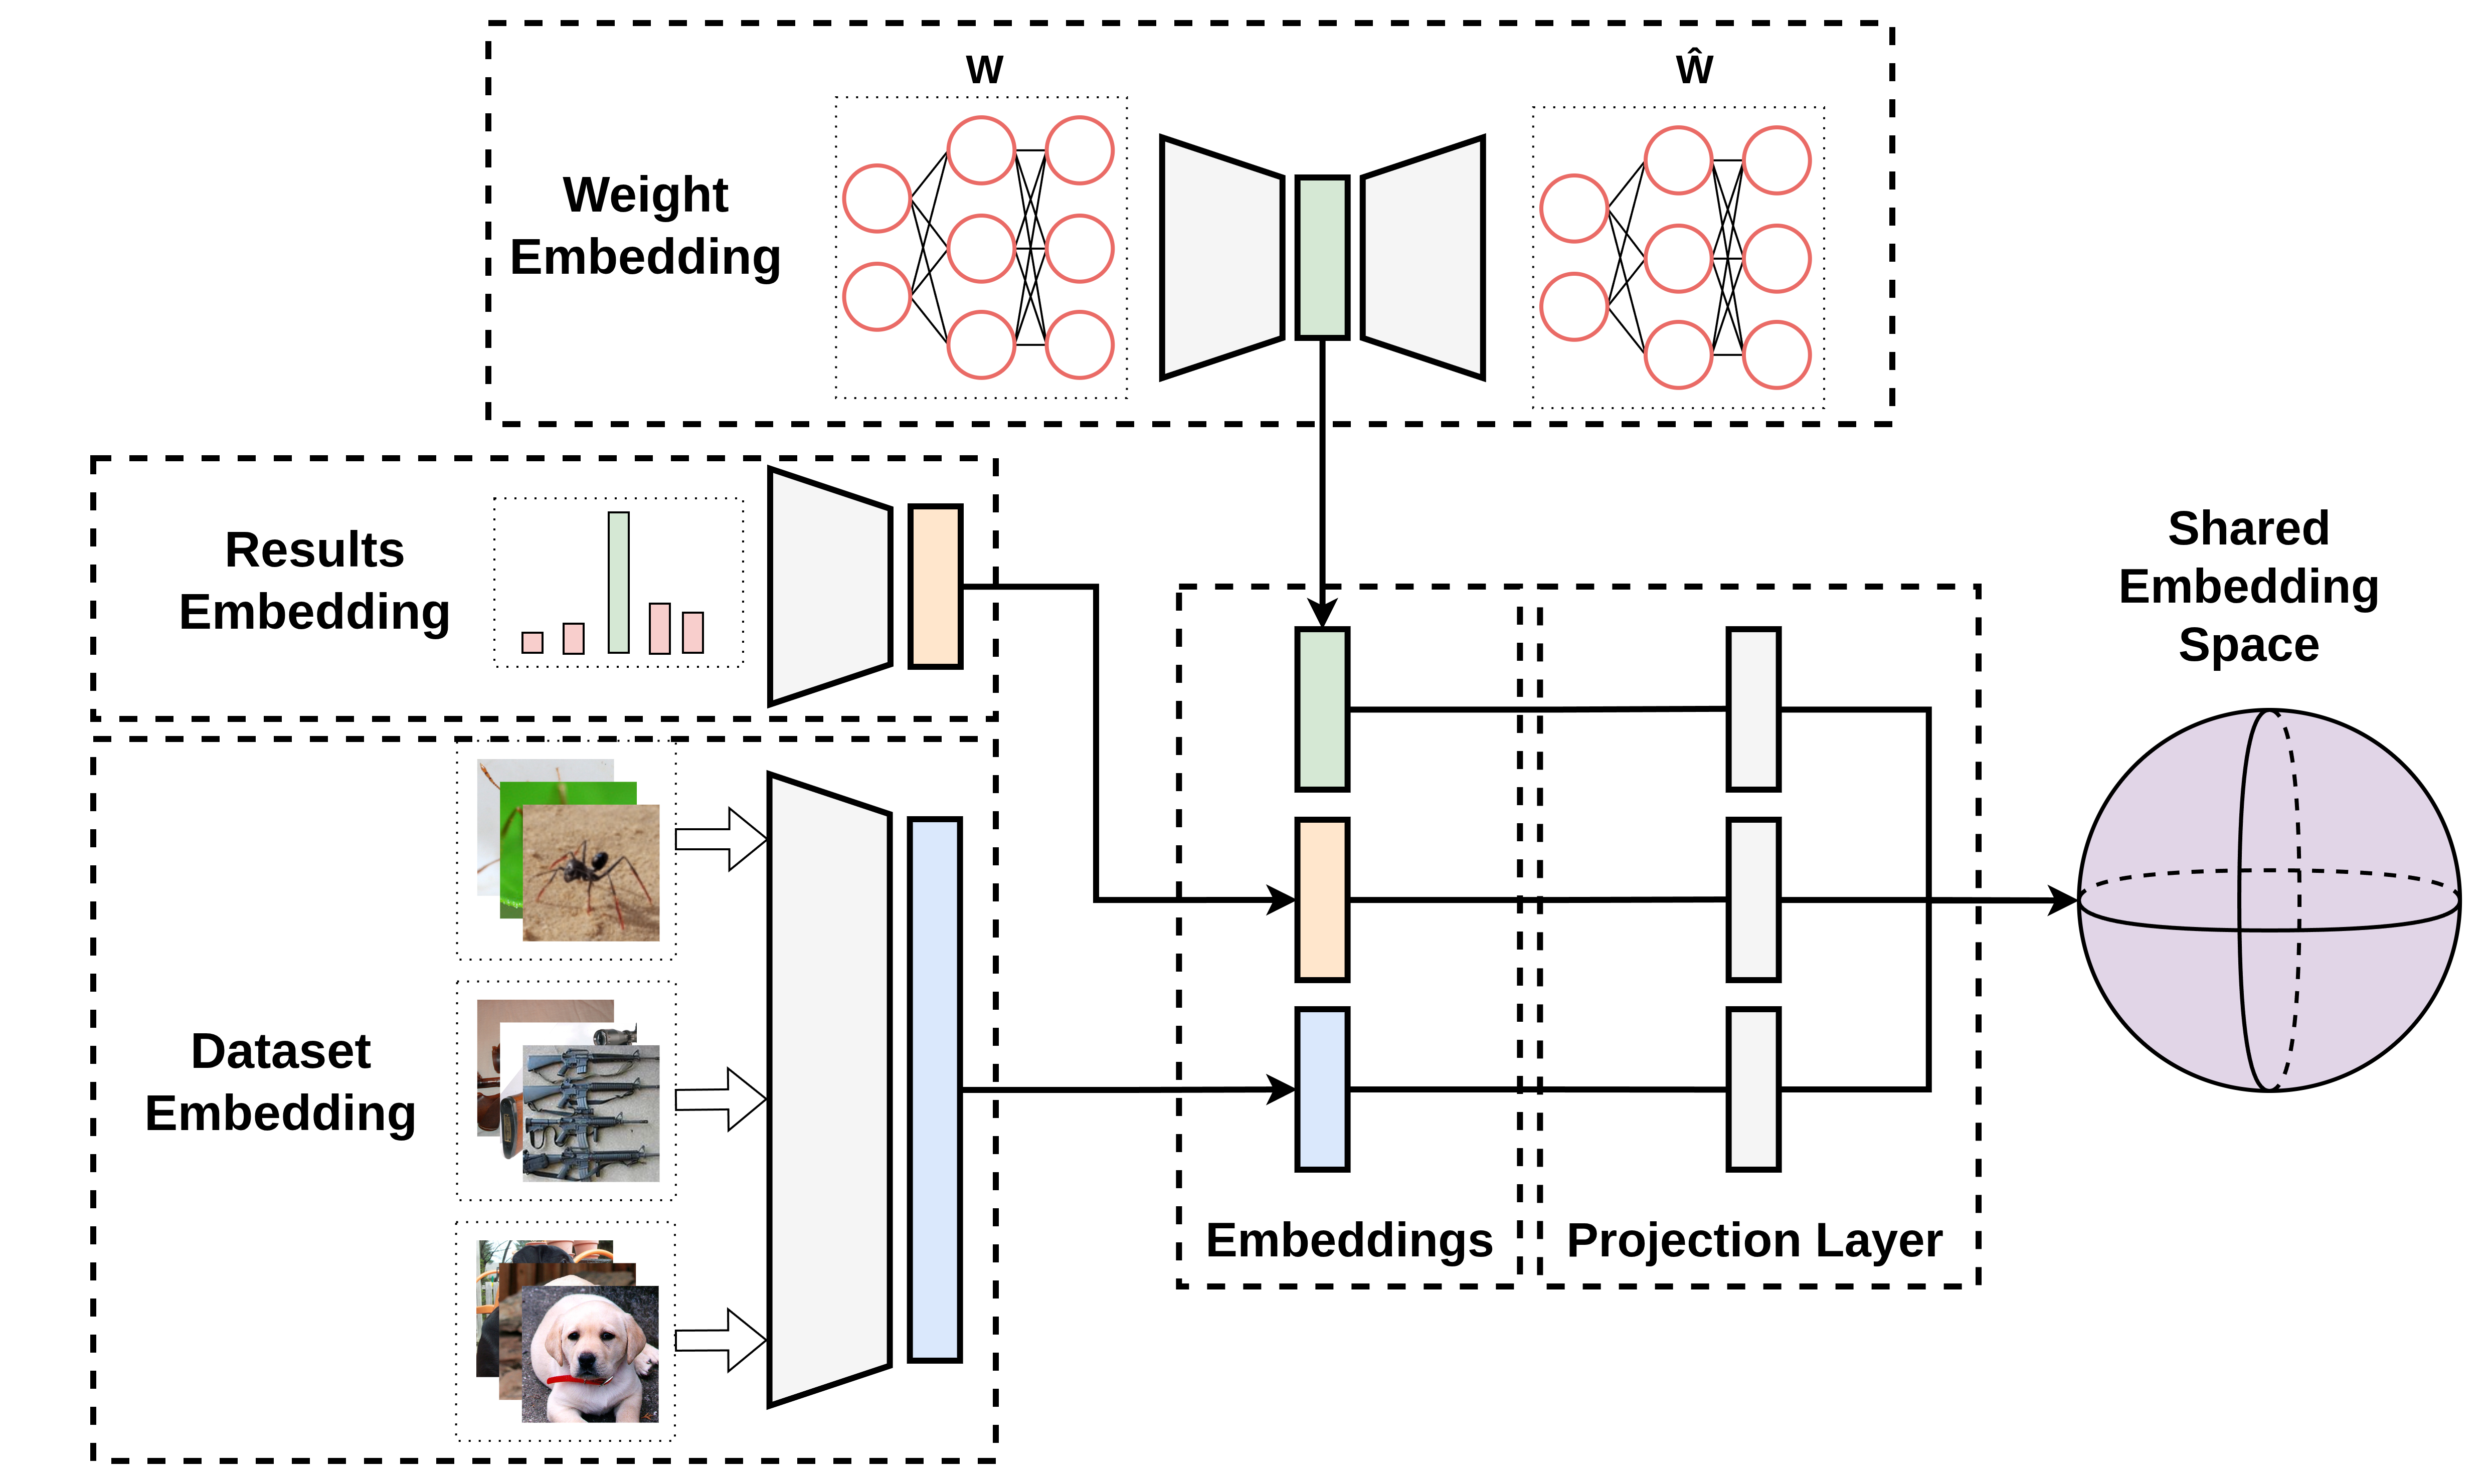
\includegraphics[width=0.75\linewidth]{pipeline.png}
    \caption[A figure illustrating the process of embedding a dataset, model weigths and results into a shared embedding space ]{AA figure illustrating the process of embedding a dataset, model weights and results in a shared embedding space. }
    \label{fig:pipeline}
\end{figure}

In this we report we develop a contrastive learning framework to create a unified embedding space that jointly represents neural network weights $(W)$, the datasets they were trained on $(\mathcal{D})$, and their resulting performance characteristics $(R)$.  Specifically, we construct two separate encoders—one for dataset embeddings using pre-trained CLIP features and one for weight embeddings using an autoencoder [cite] architecture, while creating a binned result embedding table, and train these encoders using a contrastive objective, NXTEnt \cite{agren2022ntxentlossupperbound}, that encourages related triplets $(\mathcal{D}, W, R)$ to be proximal in the shared latent space. Figure \ref{fig:pipeline} depicts a high-level view of the full embedding pipeline.

% TODO {introduction}

Our central hypothesis is that this unified representation space will enable two key capabilities:

Interpretability and Analysis: By examining the geometric relationships in the shared embedding space, we can better understand how dataset characteristics influence the learned weights and resulting model behaviors. This includes investigating questions such as: Do models trained on similar datasets cluster together in weight space? Can we identify which data characteristics most strongly determine weight patterns? 

Conditional Model Sampling: The learned distribution can enable sampling of model weights conditioned on both desired dataset properties and target performance metrics—that is, approximating P(W|D,R)—which could allow for more efficient model generation than training from scratch.







The results found from the report, and how it's limited 

The remainder of this report is structured as follows.:
    % TODO {outline_paragraph}
    In Section 1 we will discuss x, next y, concluded by z in attempt to showcase that this report is the best
    % TODO {outline_paragraph}
% TODO {introduction}


% \section{Section heading}

% This is some section with two table in it: Table~\ref{tbl:exemplars} and Table~\ref{tbl:abx_speaker}.

% \begin{table}[!h]
%     \mytable
%     \caption{Performance of the unconstrained segmental Bayesian model on TIDigits1 over iterations in which the reference set is refined.}
%     \begin{tabularx}{\linewidth}{@{}lCCCCC@{}}
%         \toprule
%         Metric     & 1 & 2 & 3 & 4 & 5 \\
%         \midrule
%         WER (\%)                        & $35.4$ & $23.5$ & $21.5$ & $21.2$ & $22.9$ \\
%         Average cluster purity (\%)       & $86.5$ & $89.7$ & $89.2$ & $88.5$ & $86.6$ \\
%         Word boundary $F$-score (\%)         & $70.6$ & $72.2$ & $71.8$ & $70.9$ & $69.4$ \\
%         Clusters covering 90\% of data   & 20             & 13 & 13 & 13 & 13 \\
%         \bottomrule
%     \end{tabularx}
%     \label{tbl:exemplars}
% \end{table}


% \begin{table}[!h]
%     \renewcommand{\arraystretch}{1.1}
%     \centering
%     \caption{A table with an example of using multiple columns.}
%     \begin{tabularx}{0.65\linewidth}{@{}lCCr@{}}
%         \toprule
%         & \multicolumn{2}{c}{Accuracy (\%)} \\
%         \cmidrule(lr){2-3}
%         Model    & Intermediate & Output & Bitrate\\
%         \midrule
%         Baseline & 27.5         & 26.4   & 116 \\
%         VQ-VAE   & 26.0         & 22.1   & 190 \\
%         CatVAE   & 28.7         & 24.3   & 215 \\
%         \bottomrule
%     \end{tabularx}
%     \label{tbl:abx_speaker}
% \end{table}

% \newpage

% This is a new page, showing what the page headings looks like, and showing how to refer to a figure like Figure~\ref{fig:cae_siamese}.

% \begin{figure}[!t]
%     \centering
% %     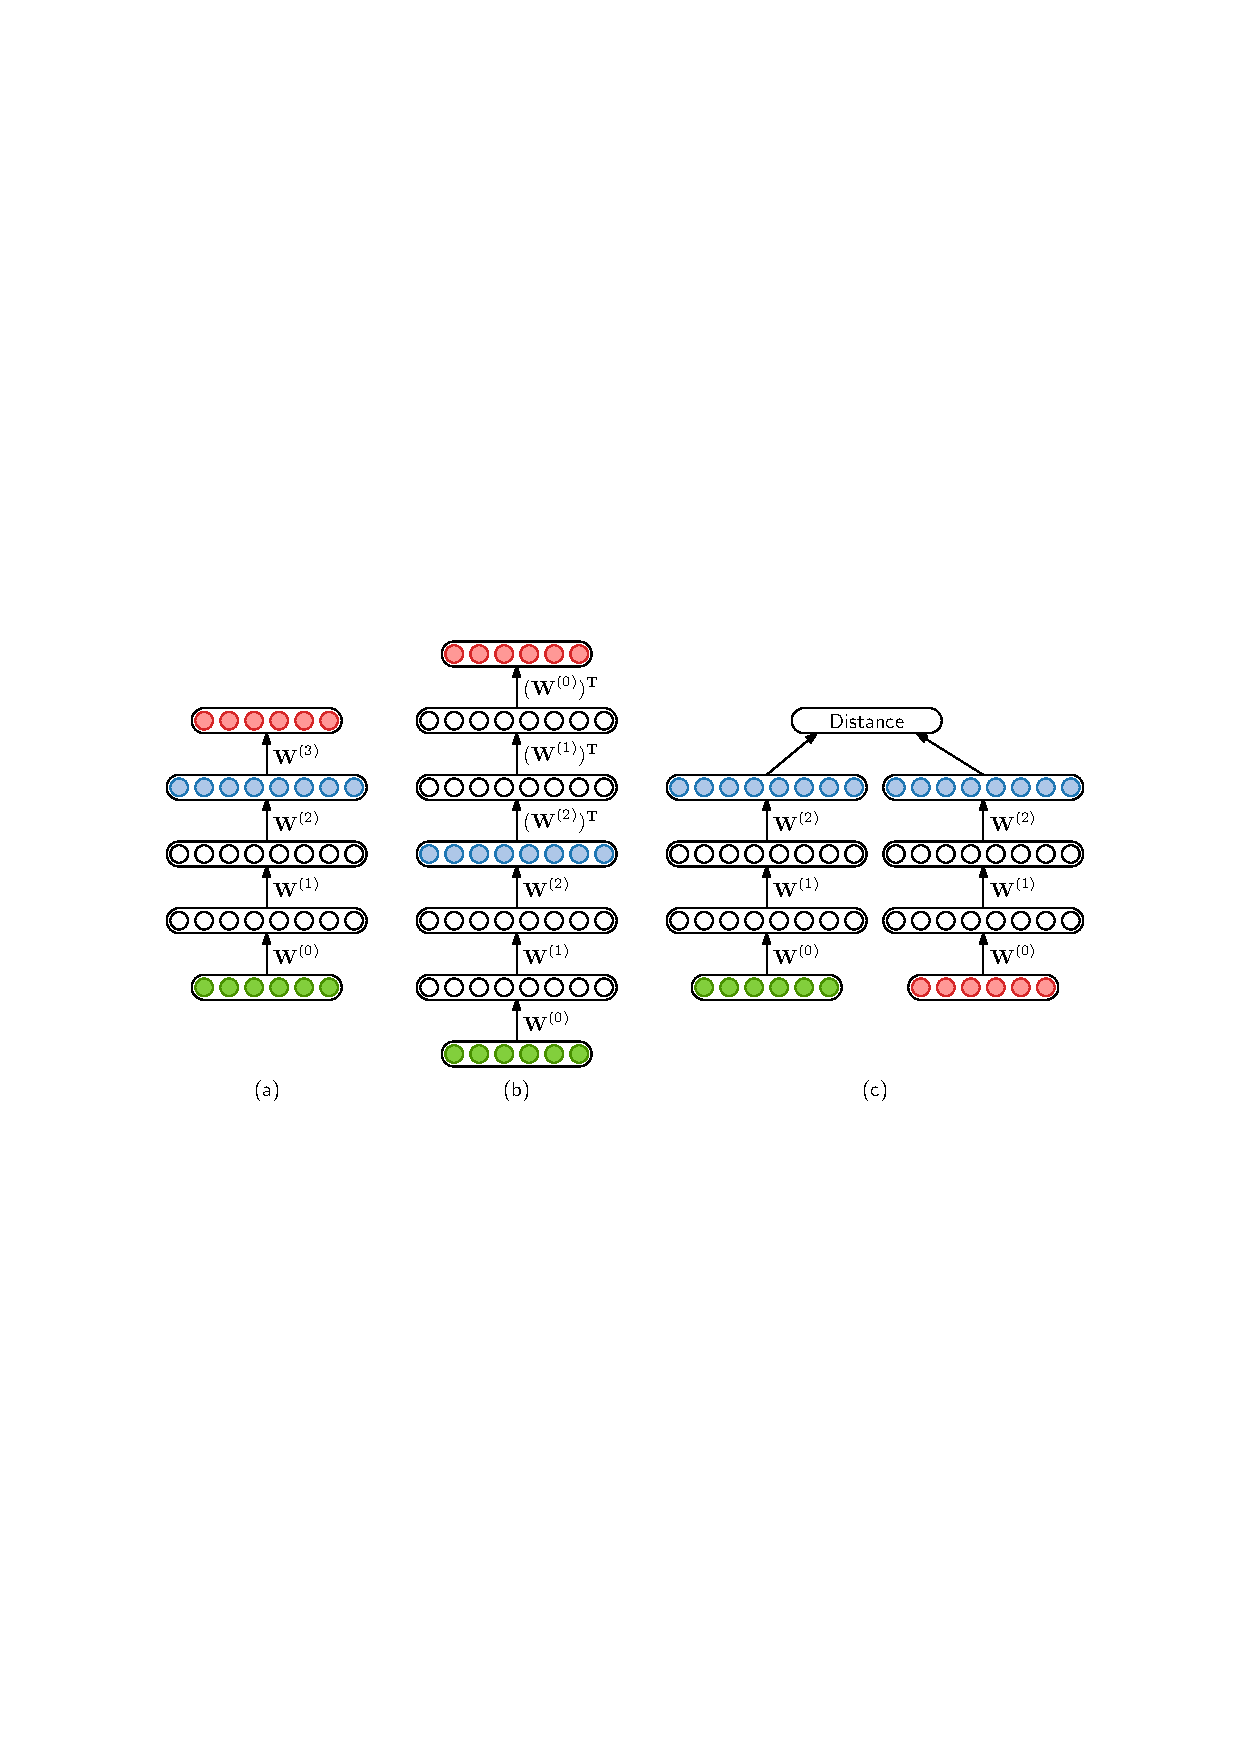
\includegraphics[width=\linewidth]{cae_siamese}
%     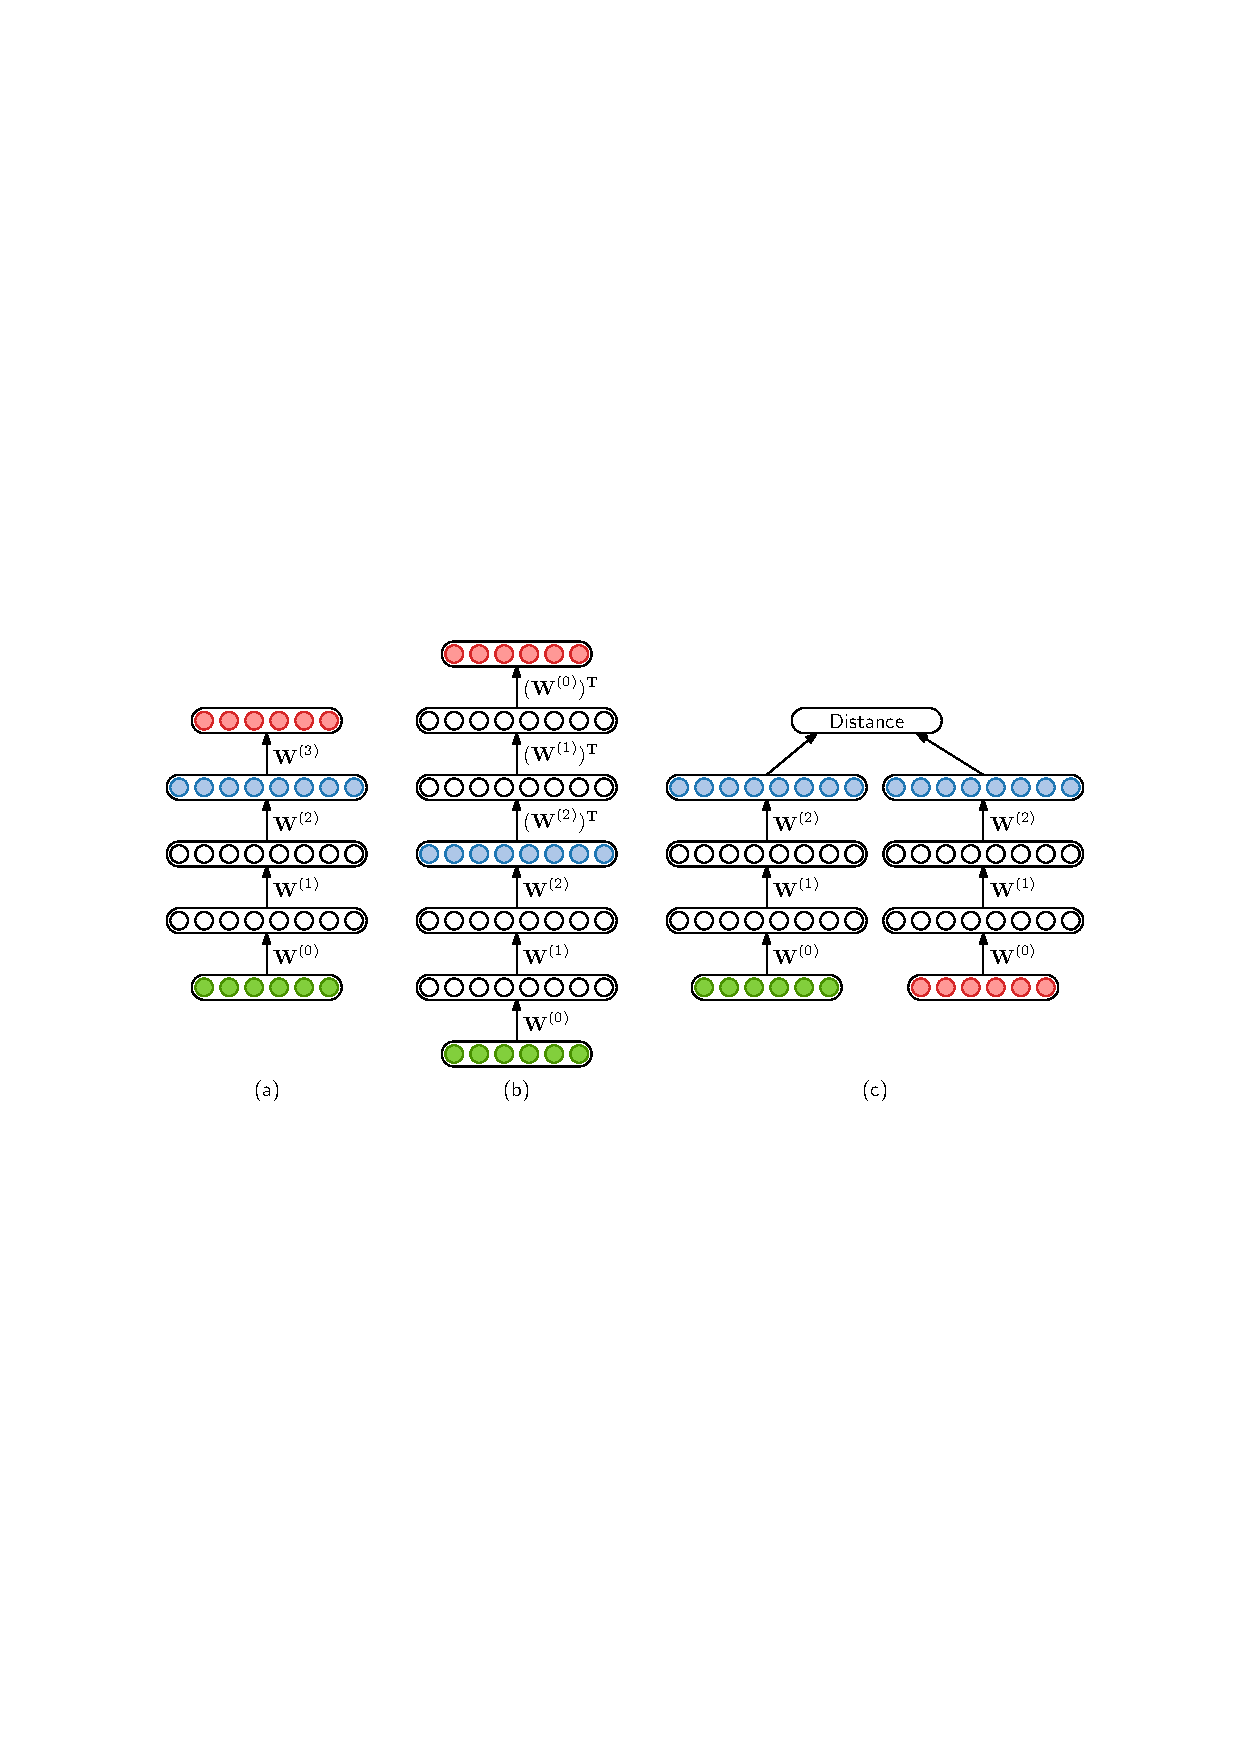
\includegraphics[width=0.918\linewidth]{cae_siamese}
%     \caption[I am the short caption that appears in the list of figures, without references.]{
%     (a) The cAE as used in this chapter. The encoding layer (blue) is chosen based on performance on a development set.
%     (b) The cAE with symmetrical tied weights. The encoding from the middle layer (blue) is always used.
%     (c) The siamese DNN. The cosine distance between aligned frames (green and red) is either minimized or maximized depending on whether the frames belong to the same (discovered) word or not.
%     A cAE can be seen as a type of DNN~\cite{dahl+etal_taslp12}.
%     }
%     \label{fig:cae_siamese}
% \end{figure}


% The following is an example of an equation:
% \begin{equation}
% P(\vec{z} | \vec{\alpha}) = \int_{\vec{\pi}} P(\vec{z} | \vec{\pi}) \, p(\vec{\pi} | \vec{\alpha}) \, \textrm{d} \vec{\pi}
% = \int_{\vec{\pi}} \prod_{k = 1}^K \pi_k^{N_k} \frac{1}{B(\vec{\alpha})} \prod_{k = 1}^K \pi_k^{\alpha_k - 1} \, \textrm{d} \vec{\pi}
% \label{eq:example_equation}
% \end{equation}
% which you can subsequently refer to as~\eqref{eq:example_equation} or Equation~\ref{eq:example_equation}.
% But make sure to consistently use the one or the other (and not mix the two ways of referring to equations).


 % include
\chapter{Background}
\label{chap:background}

% TODO {Weights Space Litarature summary}
    
% TODO {Weights Space Litarature summary}
\section{Weight Space Learning}

Weight space learning is a field within machine learning that focuses on understanding and leveraging the structure of the neural network weight space. The central aim is to model how network parameters are shaped by data, architecture, and training dynamics, and to capture these relationships within a learnable representation. 

At its core, weight space learning seeks to construct \textit{meta-models}—models that learn from other models. Unlike standard machine learning models that capture patterns in data, meta-models capture patterns in the \textit{weights} of networks trained on that data. In this way, the goal shifts from learning a direct input--output mapping to learning the structure that governs how such mappings are formed.

Due to the enormous scale and dimensionality of modern neural networks~\cite{}, it is typically infeasible to operate directly on raw model weights. Furthermore, redundancy is well known to exist in neural networks; smaller architectures can often achieve comparable performance to larger ones~\cite{}. These challenges motivate one of the central subproblems of weight space learning: the discovery of low-dimensional representations of weight space.

A \textit{latent representation} of weight space provides a compact and structured encoding of a model's parameters. The transformations—linear or non-linear—that map weights into this latent space are learned to preserve the essential information required to reconstruct or analyse the original weights. Among the many dimensionality reduction techniques available, a useful distinction can be made between \textit{reversible} and \textit{non-reversible} methods.

Reversibility is of particular importance in weight space learning. While encoding weights into a latent representation (real $\rightarrow$ latent) is informative, the ability to reconstruct the original weights (real $\rightarrow$ latent $\rightarrow$ real) is far more valuable. This reversibility enables the synthesis of entirely new weight configurations, supporting generative applications such as zero-shot model creation and performance-guided model generation. Consequently, reversible latent representation methods are the most prevalent within weight space learning, especially for encoding and decoding neural network weights.

This chapter proceeds as follows. Section~\ref{sec:pca} introduces Principal Component Analysis (PCA), a linear and probabilistic approach that provides a simple yet effective reversible dimensionality reduction method. Section~\ref{sec:autoencoders} discusses reversible, non-linear approaches, focusing on autoregressive encoder architectures and presenting the Sequential Autoencoder for Neural Embeddings (SANE)~\cite{}. Finally, Section~\ref{sec:contrastive} explores a non-reversible, modality-heterogeneous technique, contrastive learning, including a description of the NT-Xent loss and its implementation in CLIP~\cite{}.

\section{Principal Component Analysis (PCA)}
\label{sec:pca}

Principal Component Analysis (PCA) is a linear dimensionality reduction technique used to represent high-dimensional data in a lower-dimensional form while retaining as much variance as possible. It provides a compact latent representation that captures the most informative directions of variation in the data. This section outlines the motivation behind PCA, its mathematical formulation, and its relevance and limitations as a latent representation method.

\vspace{0.5em}
\noindent
\textbf{Problem Setup and Intuition.}
Consider a dataset \( X \in \mathbb{R}^{n \times d} \) with \( n \) samples and \( d \) features, centred such that each feature has zero mean. The goal of PCA is to find a new coordinate system whose axes are linear transformations of the original dimensions, ordered by the amount of variance they capture. Orthogonality between these axes ensures that each captures unique, non-redundant information about the data.

Intuitively, PCA identifies the directions that best describe the “shape” or spread of the data cloud in feature space. Projecting the data onto the top \( k \) directions provides a compressed representation that preserves most of the information while discarding redundancy.

\vspace{0.5em}
\noindent
\textbf{Mathematical Formulation.}
PCA seeks a linear projection matrix \( W \in \mathbb{R}^{d \times k} \) that maps the data to a lower-dimensional space:
\[
Z = XW,
\]
where \( Z \in \mathbb{R}^{n \times k} \) represents the latent representation.  
The sample covariance matrix of \( X \) is
\[
\Sigma = \frac{1}{n} X^\top X,
\]
and the total variance captured by the projection is
\[
\text{Var}(Z) = \text{Tr}(W^\top \Sigma W),
\]
where the trace operator \( \text{Tr}(\cdot) \) sums the variances along all projected directions.  

PCA thus maximises the variance of the projected data:
\[
\max_{W} \text{Tr}(W^\top \Sigma W)
\quad \text{subject to} \quad W^\top W = I_k.
\]
The constraint enforces orthonormality among the new axes so that each captures distinct variance. Solving this optimisation leads to the eigenvalue problem:
\[
\Sigma W = W \Lambda,
\]
where the columns of \( W \) are the eigenvectors of \( \Sigma \), and the diagonal entries of \( \Lambda \) are the corresponding eigenvalues that quantify the variance explained by each principal component. The top \( k \) eigenvectors define the optimal projection directions.

\vspace{0.5em}
\noindent
\textbf{Latent Representation and Limitations.}
The resulting embedding,

\begin{equation}
    Z = X W_k
  \label{eq:pca}
\end{equation}

is the \textit{latent representation} of the data, capturing the dominant linear structure of the dataset.  
PCA provides a reversible mapping that probabilistically preserves the greatest possible amount of variance under a linear projection. 

However, its linear nature limits its ability to capture nonlinear relationships when the data lie on curved manifolds. Furthermore, PCA does not adapt to unseen data that deviate from the original subspace—it yields a fixed, non-learnable transformation.

\vspace{0.5em}
\noindent
\textbf{Incremental PCA.}
In practice [cite], the covariance matrix \( \Sigma \) can be prohibitively large for high-dimensional data, such as neural network weights. Incremental PCA (IPCA) addresses this by processing data in smaller batches and updating the principal components iteratively. Rather than recomputing the full covariance, it approximates it using partial updates and truncated singular value decompositions (SVD).  
This approach makes IPCA suitable for large-scale or streaming datasets while maintaining results comparable to standard PCA. However, it remains an approximation and inherits PCA’s linear and non-generalisable nature.

\section{Autoencoders}
\label{sec:autoencoders}

Autoencoders are neural network architectures designed for unsupervised representation learning. Their goal is to learn a compressed, informative latent representation of input data by training the network to reconstruct the original input after passing it through a lower-dimensional bottleneck. An Autoencoder's architecture is characterized by a layer, with less nodes than the dimension of the input data, then expanding to the size of the original data. 

\vspace{0.5em}
\noindent
\textbf{Architecture and Operation.}
An autoencoder consists of two primary components: an \textit{encoder} and a \textit{decoder}. The encoder, parameterised by weights $\theta_e$, maps an input $x \in \mathbb{R}^d$ to a latent representation $z \in \mathbb{R}^k$ through a sequence of nonlinear transformations:
\begin{equation}
z = f_\text{enc}(x; \theta_e).
\label{eq:encoder}
\end{equation}
The decoder, parameterised by $\theta_d$, reconstructs the input from this latent representation:
\begin{equation}
\hat{x} = f_\text{dec}(z; \theta_d).
\label{eq:decoder}
\end{equation}
Together, the encoder and decoder form a composite function:
\begin{equation}
\hat{x} = f_\text{dec}(f_\text{enc}(x)).
\label{eq:composite}
\end{equation}
The bottleneck layer (latent space) enforces a compression constraint, ensuring the model retains only the most salient features necessary for accurate reconstruction.

\vspace{0.5em}
\noindent
\textbf{Training Objective.}
The network is trained to minimise the reconstruction error between the input $x$ and its reconstruction $\hat{x}$. The most common loss function is the Mean Squared Error (MSE):
\begin{equation}
\mathcal{L} = \frac{1}{n} \sum_{i=1}^{n} \| x_i - \hat{x}_i \|^2.
\label{eq:ae_mse_loss}
\end{equation}
This loss is automatically differentiated and optimised through backpropagation using gradient descent. By minimising this objective, the autoencoder learns weight configurations that best compress and reconstruct the data distribution.

The objective can be extended to include additional terms depending on the desired properties of the latent space. For example, a \textit{contrastive loss} component can be incorporated to encourage semantic separation between latent representations, improving feature discriminability. Likewise, \textit{regularisation} terms—such as $L_1$ or $L_2$ penalties, or sparsity constraints—can be added to improve generalisation and prevent overfitting by controlling the magnitude or distribution of learned weights.


\vspace{0.5em}
\noindent
\textbf{Latent Representation and Flexibility.}
The latent space $z$ provides a nonlinear embedding that captures underlying structure within the data. Once trained, the encoder can be used independently for dimensionality reduction or feature extraction, while the decoder can serve as a generative mapping from the latent space back to the input domain.

Autoencoders are highly flexible in architecture — they can be shallow for simple data or deep to capture hierarchical structure. Nonlinear activation functions such as ReLU, tanh, or sigmoid increase expressivity, allowing the model to represent complex, nonlinear manifolds within the data distribution.

\subsection{Autoencoder for Neural Embeddings}
Applying the concept of an autoencoder to neural network weights has recently gained attention as a means to learn structured, low-dimensional representations of model parameters. Instead of encoding raw input data, the autoencoder learns to encode and reconstruct the weights of pre-trained neural networks, effectively embedding each model into a latent space that captures structural and functional similarities between models. This approach was explored in \cite{NEURIPS2022_b2c4b7d3}, where the goal was to build a continuous and interpretable representation space of neural weights.

\vspace{0.5em}
\noindent
\textbf{Training Objective.}
Unlike conventional autoencoders that optimise a single reconstruction loss, the neural weight autoencoder is trained with a multi-objective loss function that combines reconstruction and contrastive terms:
\begin{equation}
\mathcal{L} = \beta \mathcal{L}_{\text{MSE}} + (1 - \beta) \mathcal{L}_{\text{c}},
\label{eq:multi_loss}
\end{equation}
where $\mathcal{L}_{\text{MSE}}$ represents the weight reconstruction loss and $\mathcal{L}_{\text{c}}$ is a contrastive loss.  
The reconstruction term encourages the decoder to accurately reproduce the original model weights, expressed layer-wise as:
\begin{equation}
\mathcal{L}_{\text{MSE}} = \frac{1}{MN} \sum_{i=1}^{M} \sum_{l=1}^{L} \| \hat{w}_i^{(l)} - w_i^{(l)} \|_2^2,
\label{eq:weight_recon_loss}
\end{equation}
where $w_i^{(l)}$ and $\hat{w}_i^{(l)}$ are the original and reconstructed weights for the $l$-th layer of the $i$-th model in the collection (often called a \textit{model zoo}).  

The contrastive component $\mathcal{L}_{\text{c}}$ introduces additional structure in the latent space by applying data augmentations during training—such as weight permutation (which leverages inherent symmetries in neural networks) and random erasing—to ensure that semantically similar models are mapped closer together while dissimilar ones are pushed apart. In this work, the contrastive term follows the \textit{NXTne} loss formulation (see Section~\ref{sec:nxtne_loss}), which provides a more stable and expressive contrastive objective for modelling relationships in weight space.


This combination of reconstruction and contrastive learning encourages the encoder to capture not only numerical similarity in the weights but also functional and architectural relationships between models. The result is a structured latent space in which proximity correlates with similarity in performance or behaviour.

\vspace{0.5em}
\noindent
\textbf{Interpretation and Utility.}
The learned latent space enables both discriminative and generative applications. The encoder can be used to extract informative embeddings that summarise a model’s functional behaviour, useful for clustering, transfer learning, or model retrieval. Meanwhile, the decoder can generate entirely new sets of weights from latent vectors—supporting generative applications such as zero-shot model synthesis or interpolation between models. This dual capability makes the autoencoder framework particularly appealing for weight space learning, as it provides both interpretability and controllability.

\vspace{1em}
\noindent
\textbf{Sequential Autoencoder for Neural Embeddings.}
A major challenge in encoding neural network weights lies in the enormous number of parameters, which quickly becomes infeasible to process directly. \cite{pmlr-v235-schurholt24a} introduced the Sequential Autoencoder for Neural Embeddings (SANE), which addresses this scalability problem by tokenising model weights rather than treating the entire parameter set as a single input.  

Instead of encoding full weight tensors, SANE partitions them into smaller, semantically meaningful \textit{tokens}—for example, by layer or even within layers—and encodes these sequentially. Each token is represented as a point in latent space, and the entire model is represented as a \textit{cloud of latent tokens} rather than a single vector. This design assumes that sufficient information about the model’s global behaviour is preserved through these local token representations, an assumption supported by empirical results in \cite{pmlr-v235-schurholt24a}.

SANE achieves state-of-the-art performance in both discriminative and generative weight-space applications, demonstrating that this token-based decomposition maintains the essential structure of models while dramatically improving scalability. Furthermore, because the approach is sequential, it naturally accommodates heterogeneous architectures—normalising across different layer types and sizes—and allows the generation of new architectures by decoding variable-length token sequences.  

This flexibility marks an important step toward scalable and architecture-agnostic representation learning in weight space.

\section{Contrastive Learning}
\label{sec:contrastive}
The overall goal of contrastive learning is to learn meaningful representations by comparing data points against one another, rather than relying on explicit labels \cite{}. The foundational assumption is that if a model is provided with sufficient examples of similar and dissimilar pairs, it can learn to represent data such that semantically similar samples lie close together in the embedding space, while dissimilar samples are placed farther apart. This framework enables unsupervised or self-supervised learning of latent representations that capture semantic structure purely through relative similarity.

\subsection{NT-Xent Loss}
\label{sec:nxtne_loss}
A widely used objective for contrastive learning is the Normalised Temperature-Scaled Cross Entropy (NT-Xent) loss introduced in \cite{}. This loss formulates the contrastive task as a classification problem over positive and negative pairs within a batch.  
Given a batch of $N$ samples, each with an augmented pair $(x_i, x_i')$, the loss for a positive pair $(i, j)$ is defined as:
\begin{equation}
  \mathcal{L}_{i,j} = -\log \frac{\exp(\text{sim}(z_i, z_j) / \tau)}{\sum_{k=1}^{2N} \mathbb{1}_{[k \neq i]} \exp(\text{sim}(z_i, z_k) / \tau)}
  \label{eq:nt-xent_loss}
\end{equation}
where $\text{sim}(z_i, z_j)$ denotes the cosine similarity between the latent representations $z_i$ and $z_j$, and $\tau$ is a temperature parameter that controls the sharpness of the distribution. The total batch loss is obtained by averaging over all positive pairs.  
This formulation encourages positive pairs (augmentations of the same sample) to have high similarity, while simultaneously pushing apart embeddings from different samples, resulting in well-structured and discriminative latent representations.

\subsection{CLIP}
An important application of contrastive learning using the NT-Xent objective is CLIP (Contrastive Language--Image Pretraining) \cite{}. CLIP jointly trains an image encoder and a text encoder to align visual and textual representations in a shared embedding space.  
During training, each image is paired with a corresponding caption, forming a positive pair, while all other image--text combinations in the batch act as negatives. The model optimises a symmetric contrastive objective, where each image predicts its matching caption and vice versa:
\[
\mathcal{L}_{\text{CLIP}} = \frac{1}{2}(\mathcal{L}_{\text{image-to-text}} + \mathcal{L}_{\text{text-to-image}}).
\]
Through this process, CLIP learns general-purpose visual and linguistic representations that are semantically aligned. Once trained, the model can perform zero-shot classification and other cross-modal tasks by measuring similarity between image and text embeddings without task-specific fine-tuning. % include
\chapter{Methodology} % include
\chapter{Results and Analysis} % include
\graphicspath{{conclusion/fig/}}

\chapter{Summary and Conclusion}
\label{chap:conclusion} % include



% \begin{table}[!h]
%     \mytable
%     \caption{}
%     \begin{tabularx}{\linewidth}{@{}lCCCCC@{}}
%         \toprule
%         Metric     & 1 & 2 & 3 & 4 & 5 \\
%         \midrule
%         WER (\%)                        & $35.4$ & $23.5$ & $21.5$ & $21.2$ & $22.9$ \\
%         Average cluster purity (\%)       & $86.5$ & $89.7$ & $89.2$ & $88.5$ & $86.6$ \\
%         Word boundary $F$-score (\%)         & $70.6$ & $72.2$ & $71.8$ & $70.9$ & $69.4$ \\
%         Clusters covering 90\% of data   & 20             & 13 & 13 & 13 & 13 \\
%         \bottomrule
%     \end{tabularx}
%     \label{tbl:exemplars}
% \end{table}


% \begin{table}[!h]
%     \renewcommand{\arraystretch}{1.1}
%     \centering
%     \caption{A table with an example of using multiple columns.}
%     \begin{tabularx}{0.65\linewidth}{@{}lCCr@{}}
%         \toprule
%         & \multicolumn{2}{c}{Accuracy (\%)} \\
%         \cmidrule(lr){2-3}
%         Model    & Intermediate & Output & Bitrate\\
%         \midrule
%         Baseline & 27.5         & 26.4   & 116 \\
%         VQ-VAE   & 26.0         & 22.1   & 190 \\
%         CatVAE   & 28.7         & 24.3   & 215 \\
%         \bottomrule
%     \end{tabularx}
%     \label{tbl:abx_speaker}
% \end{table}

% Bibliography
\bibliography{mybib} % include

% End matter
% \appendix
% \chapter{Project Planning Schedule}
\makeatletter\@mkboth{}{Appendix}\makeatother
\label{appen:derivations_bigramseg}

This is an appendix.

\chapter{Outcomes Compliance}
\makeatletter\@mkboth{}{Appendix}\makeatother
% \label{appen:derivations_bigramseg}

This is another appendix.

\end{document}

